\documentclass[11pt]{article}

\usepackage[margin=0.85in]{geometry}
\usepackage[T1]{fontenc}
\usepackage[utf8]{inputenc}
\usepackage{lmodern}
\usepackage{microtype}
\usepackage{graphicx}
\usepackage{booktabs}
\usepackage{array}
\usepackage{amsmath}
\usepackage{amssymb}
\usepackage{hyperref}
\usepackage{xcolor}
\usepackage{caption}
\usepackage{subcaption}
\usepackage{float}

\hypersetup{
  colorlinks=true,
  linkcolor=blue,
  citecolor=blue,
  urlcolor=blue
}

\newcommand{\projectroot}{/home/lachlan/ProjectsLFS/OrganoidAgent}
\newcommand{\outputroot}{/home/lachlan/ProjectsLFS/OrganoidAgent/analysis-outputs/yichao_future_expression}
\newcommand{\metric}[1]{\textbf{#1}}

\title{\textbf{Projected Brightfield-to-Fluorescence and Early Future Expression Prediction in Yichao Organoid Time Series}}
\author{OrganoidAgent analysis report}
\date{May 11, 2026}

\begin{document}
\maketitle

\begin{abstract}
This technical report summarizes the completed Yichao projected-organoid prediction experiments and incorporates the generated quantitative outputs, prediction panels, and feature-explanation visualizations. The first task tests same-time brightfield-to-fluorescence prediction, denoted $B_t \rightarrow F_t$, using complete non-edge projected organoid instances. This task is feasible: the held-out test split achieves image mean absolute error (MAE) of 0.1077, positive-expression AUROC of 0.728, and fluorescence-peak Pearson correlation of 0.685. The second task tests early future-expression prediction from brightfield history, denoted $B_{0:k} \rightarrow F_{p>k}$. The scalar-only future model is weak on the held-out test split (future-positive AUROC 0.228, future-peak Pearson 0.134), so it should be treated as a baseline rather than a usable predictor. A joint model combining auxiliary same-time B2F with dense future fluorescence prediction also fails to generalize on the held-out future test split (future-positive AUROC 0.223, future-peak Pearson -0.049). Feature analysis nevertheless indicates that projected organoid size, bounding-box dimensions, segmentation support ratio, and boundary strength are the strongest explicit morphology signals for same-time fluorescence distinction.
\end{abstract}

\section{Data and Output Scope}

All results in this report use the projected complete/non-edge Yichao instance dataset prepared from the projected instance database:

\begin{center}
\small
\path{/home/lachlan/ProjectsLFS/OrganoidAgent/analysis-outputs/yichao_future_expression/future_expression.sqlite}
\end{center}

The materialized dataset contains 9,380 projected complete/non-edge instances, 363 linked time-series tracks, and 6,088 early-prefix future samples. Future samples are split into 4,277 train, 1,178 validation, and 633 held-out test examples.

\begin{table}[H]
\centering
\caption{Main output directories incorporated into this report.}
\begin{tabular}{p{0.24\linewidth}p{0.68\linewidth}}
\toprule
Output type & Path \\
\midrule
B2F evaluation & \path{\outputroot/stage1_b2f_evaluation} \\
Feature explanation & \path{\outputroot/stage1_feature_analysis} \\
Scalar future baseline & \path{\outputroot/stage2_future_expression} \\
Consolidated previous run & \path{\outputroot/previous_run_evaluation} \\
Joint B2F/future run & \path{\outputroot/stage3_joint_b2f_future} \\
\bottomrule
\end{tabular}
\end{table}

\section{Mathematical Formulation}

For each projected organoid instance at time $t$, the dataset provides a brightfield crop $B_t \in \mathbb{R}^{1 \times H \times W}$, a fluorescence crop $F_t \in \mathbb{R}^{1 \times H \times W}$, and an organoid mask $M_t \in \{0,1\}^{1 \times H \times W}$. The same-time feasibility model learns
\begin{equation}
\hat{F}_t = G_{\theta}(B_t),
\end{equation}
with a masked reconstruction loss
\begin{equation}
\mathcal{L}_{\mathrm{img}}(\hat{F},F,M)
= \mathrm{mean}(|\hat{F}-F|M)
+ \lambda_{\mathrm{bg}}\mathrm{mean}(|\hat{F}-F|(1-M)),
\end{equation}
where $\lambda_{\mathrm{bg}}=0.2$.

The future-expression problem uses a prefix of brightfield observations,
\begin{equation}
P_k = \{(B_j, X_j, v_j)\}_{j=k-L+1}^{k},
\end{equation}
where $X_j$ is a vector of explicit morphology/time features and $v_j$ indicates valid prefix frames. The future task is
\begin{equation}
(\hat{F}_p,\hat{a}_p,\hat{r}_p,\hat{q}_p)
= H_{\phi}(P_k), \quad p>k,
\end{equation}
where $\hat{F}_p$ is a predicted future fluorescence image, $\hat{a}_p$ is the future-positive logit, $\hat{r}_p$ is the predicted future peak fluorescence, and $\hat{q}_p$ is the predicted future fluorescence AUC.

The proposed joint objective is
\begin{equation}
\mathcal{L}
= \mathcal{L}_{\mathrm{img}}(\hat{F}_p,F_p,M_p)
+ \gamma\mathcal{L}_{\mathrm{img}}(\hat{F}_k,F_k,M_k)
+ \eta\mathcal{L}_{\mathrm{scalar}},
\end{equation}
where the auxiliary $B_k \rightarrow F_k$ branch regularizes the future model with the already validated same-time B2F signal.

\section{Headline Results}

\begin{figure}[H]
\centering
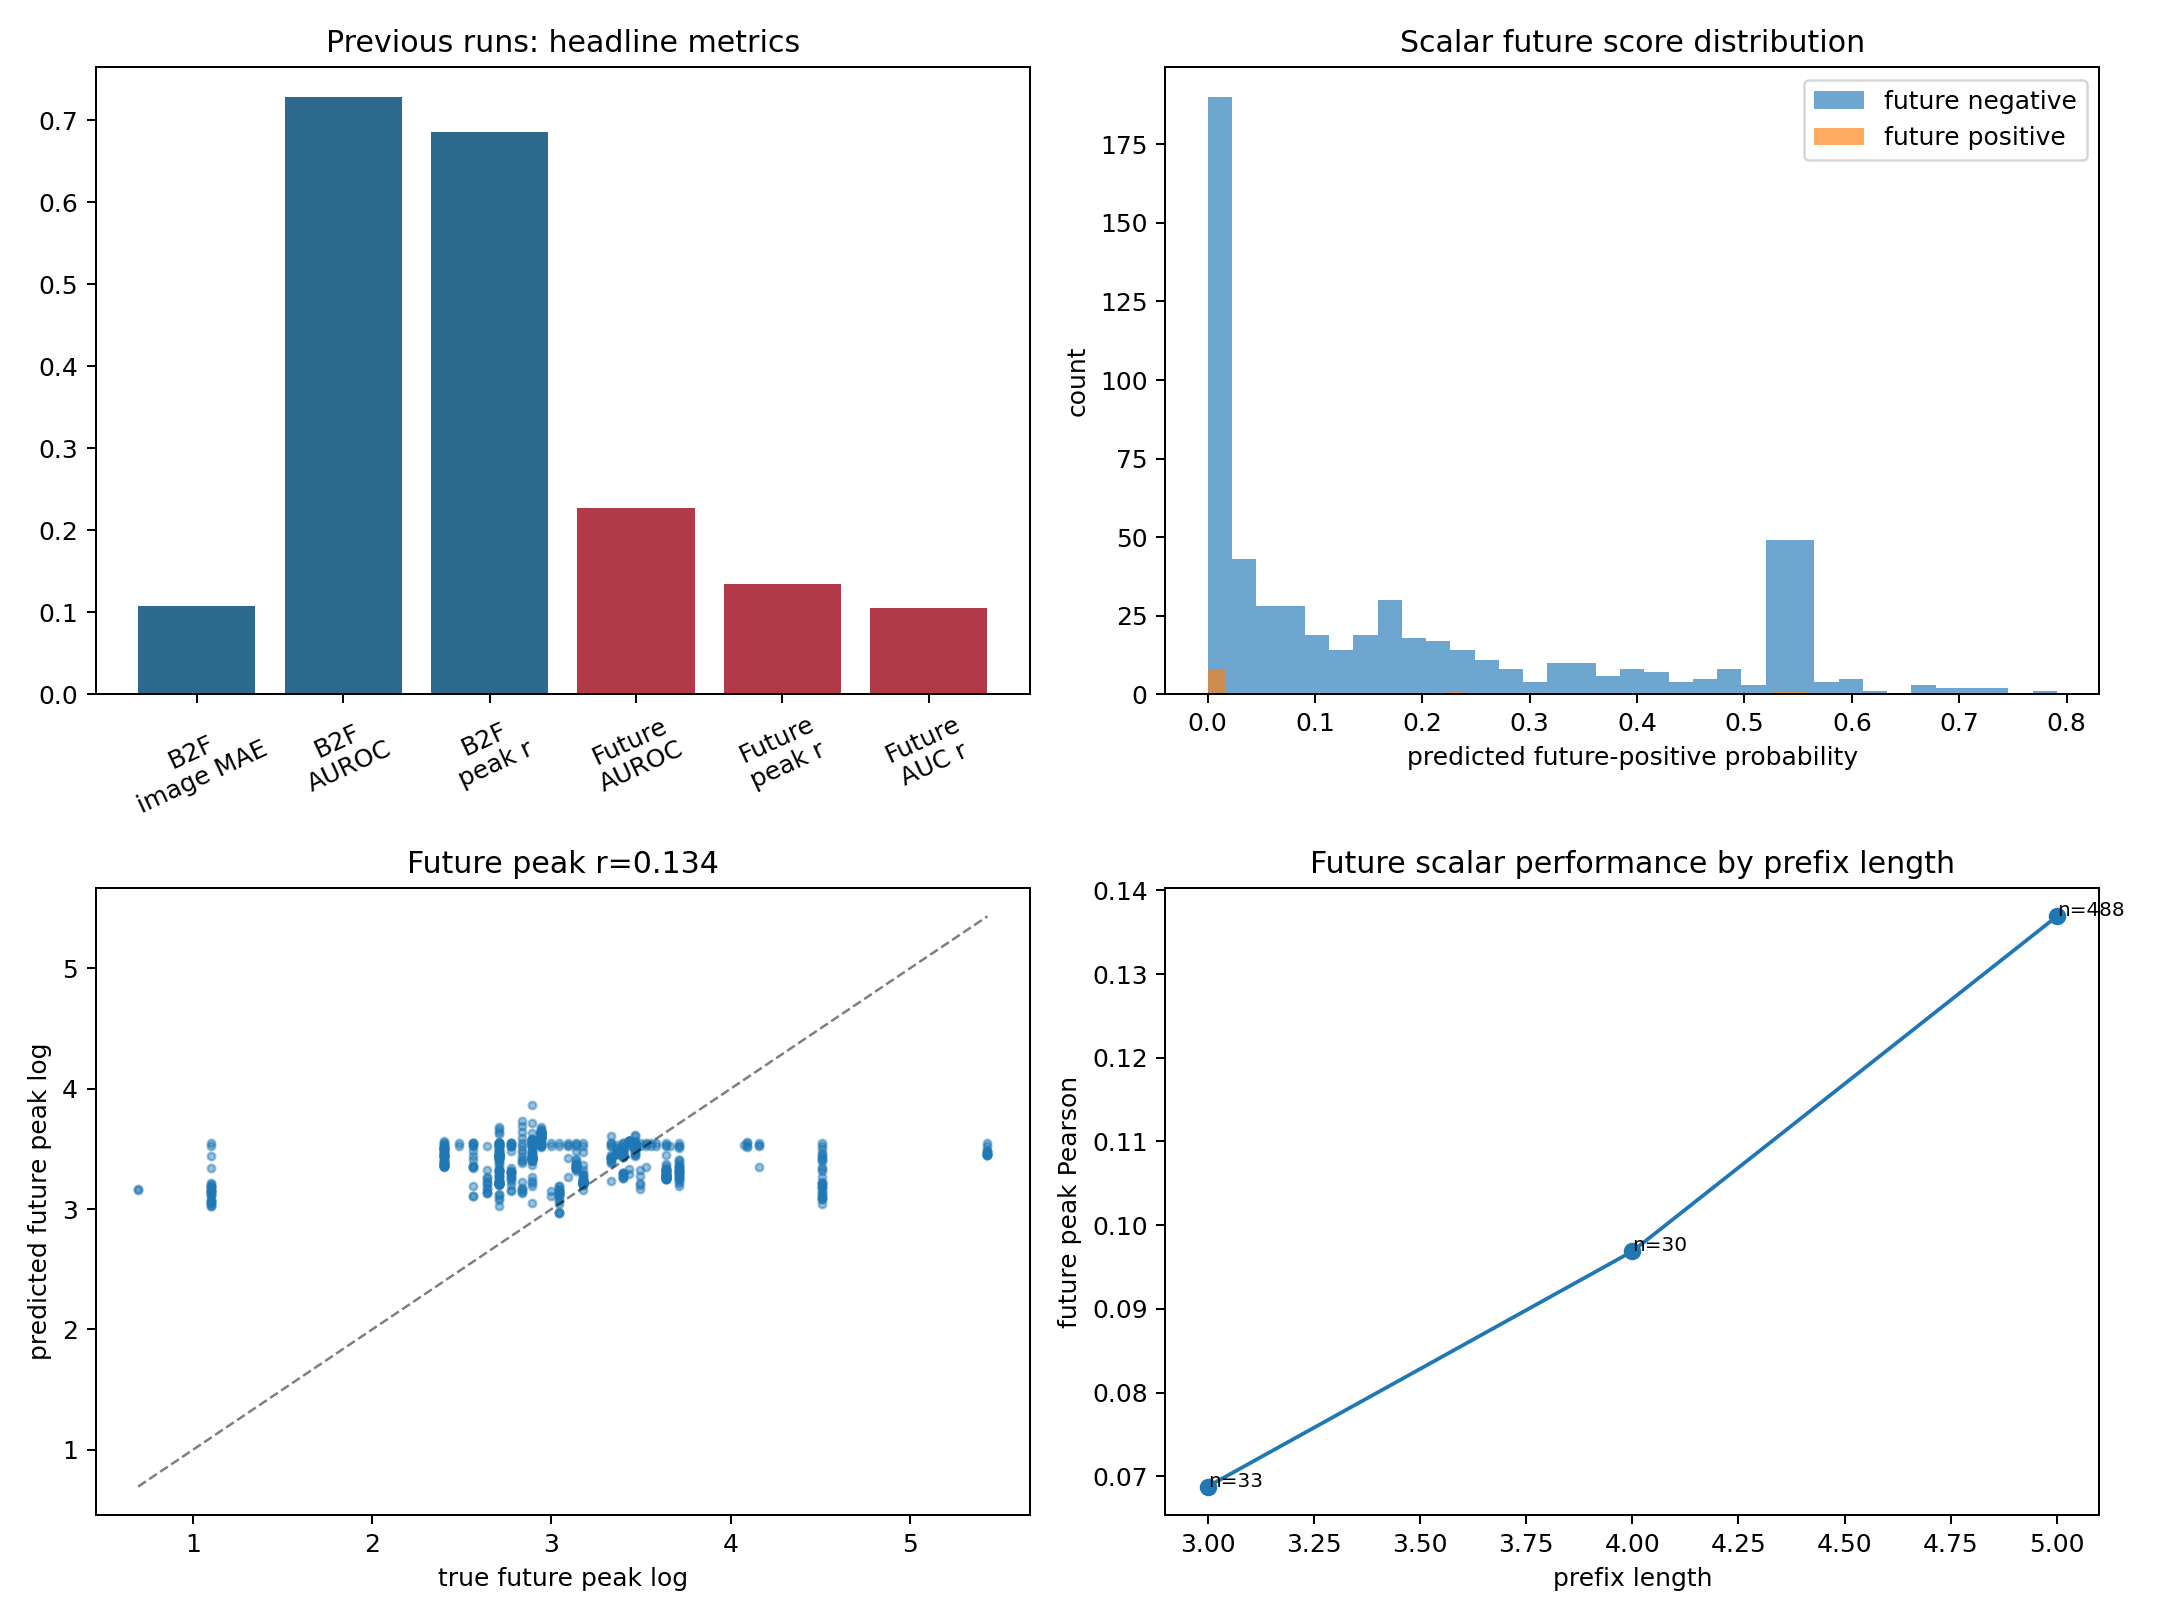
\includegraphics[width=\linewidth]{figures/fig1_previous_run_overview.png}
\caption{Consolidated overview of completed previous runs. The panel combines same-time B2F headline metrics, future scalar score separation, future peak prediction scatter, and prefix-length behavior for the scalar future baseline.}
\label{fig:previous-overview}
\end{figure}

\begin{table}[H]
\centering
\caption{Held-out test metrics for completed prediction runs.}
\begin{tabular}{lccc}
\toprule
Metric & Same-time B2F & Scalar future & Joint B2F/future \\
\midrule
Held-out test examples & 1,088 & 633 & 633 \\
Positive examples & 14 & not fixed in metric file & 11 \\
Image MAE & 0.1077 & not predicted & 0.3112 \\
Image PSNR & 14.18 dB & not predicted & 7.95 dB \\
Positive AUROC & 0.728 & 0.228 & 0.223 \\
Average precision & 0.110 & 0.0156 & 0.0127 \\
Peak Pearson correlation & 0.685 & 0.134 & -0.049 \\
AUC Pearson correlation & not applicable & 0.105 & 0.075 \\
\bottomrule
\end{tabular}
\end{table}

The same-time B2F result supports feasibility: projected brightfield morphology contains useful information for reconstructing contemporaneous fluorescence structure and estimating fluorescence intensity. The scalar future and joint future models do not yet support reliable early future prediction on the held-out test split. They are retained as negative baselines and as diagnostics for future data/target design.

\section{Same-Time Brightfield-to-Fluorescence Feasibility}

\begin{figure}[H]
\centering
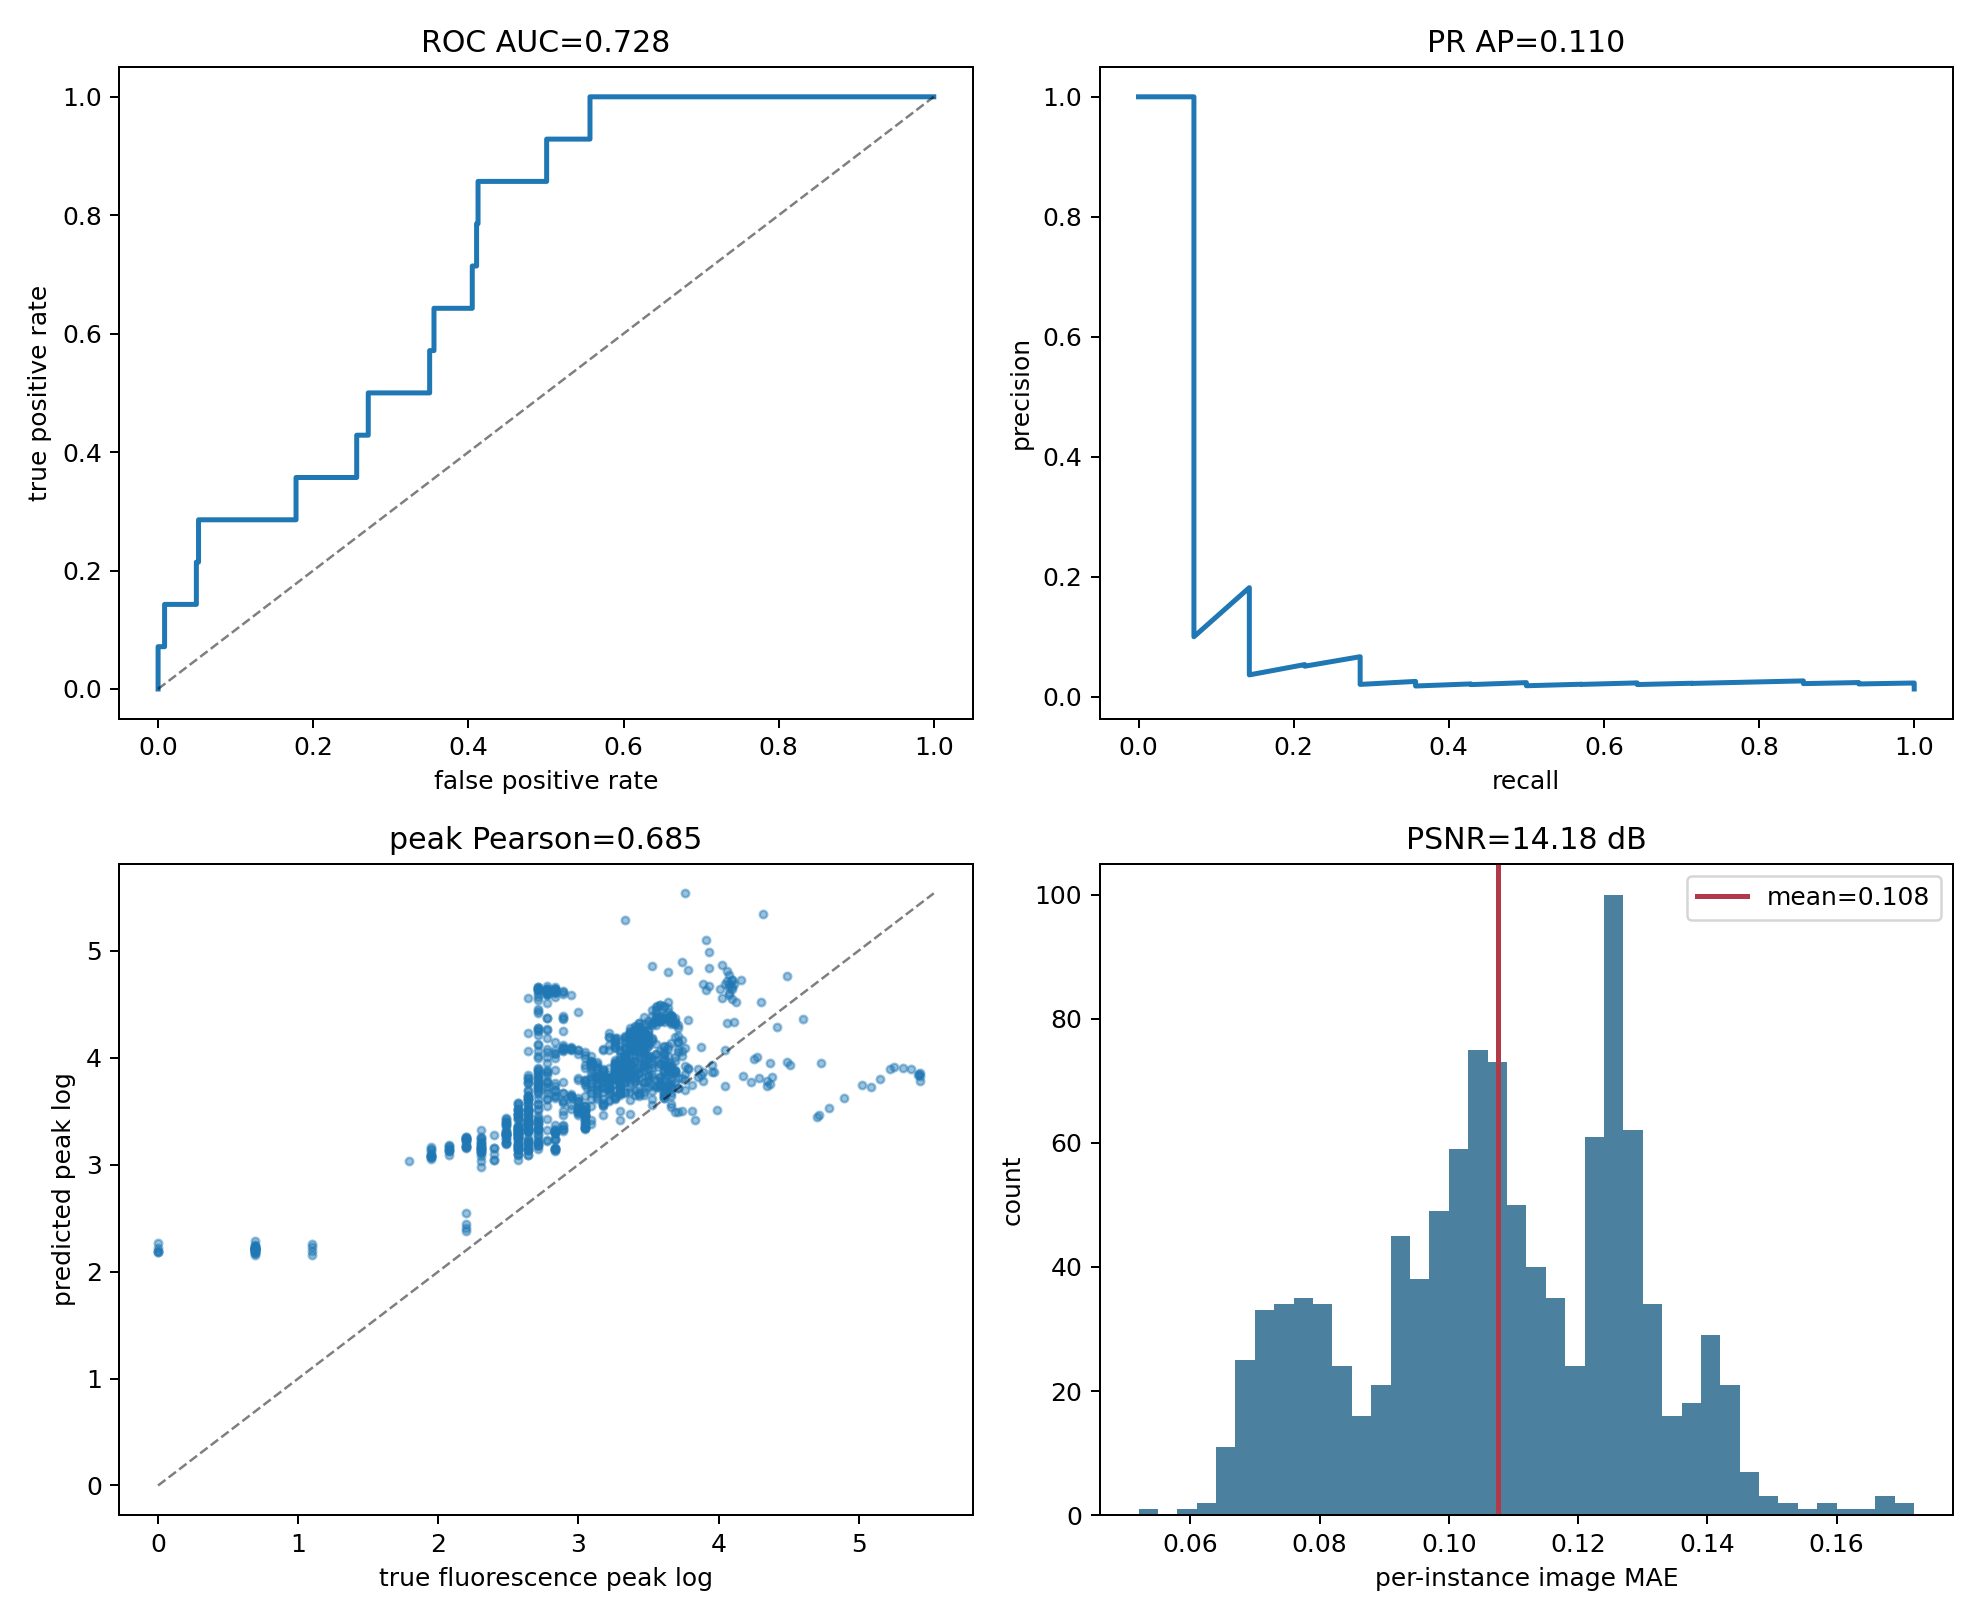
\includegraphics[width=\linewidth]{figures/fig2_b2f_performance_summary.png}
\caption{B2F held-out performance summary. The figure contains ROC/PR behavior for fluorescence positivity, predicted-versus-true fluorescence peak correlation, and per-instance image error distribution.}
\label{fig:b2f-summary}
\end{figure}

\begin{figure}[H]
\centering
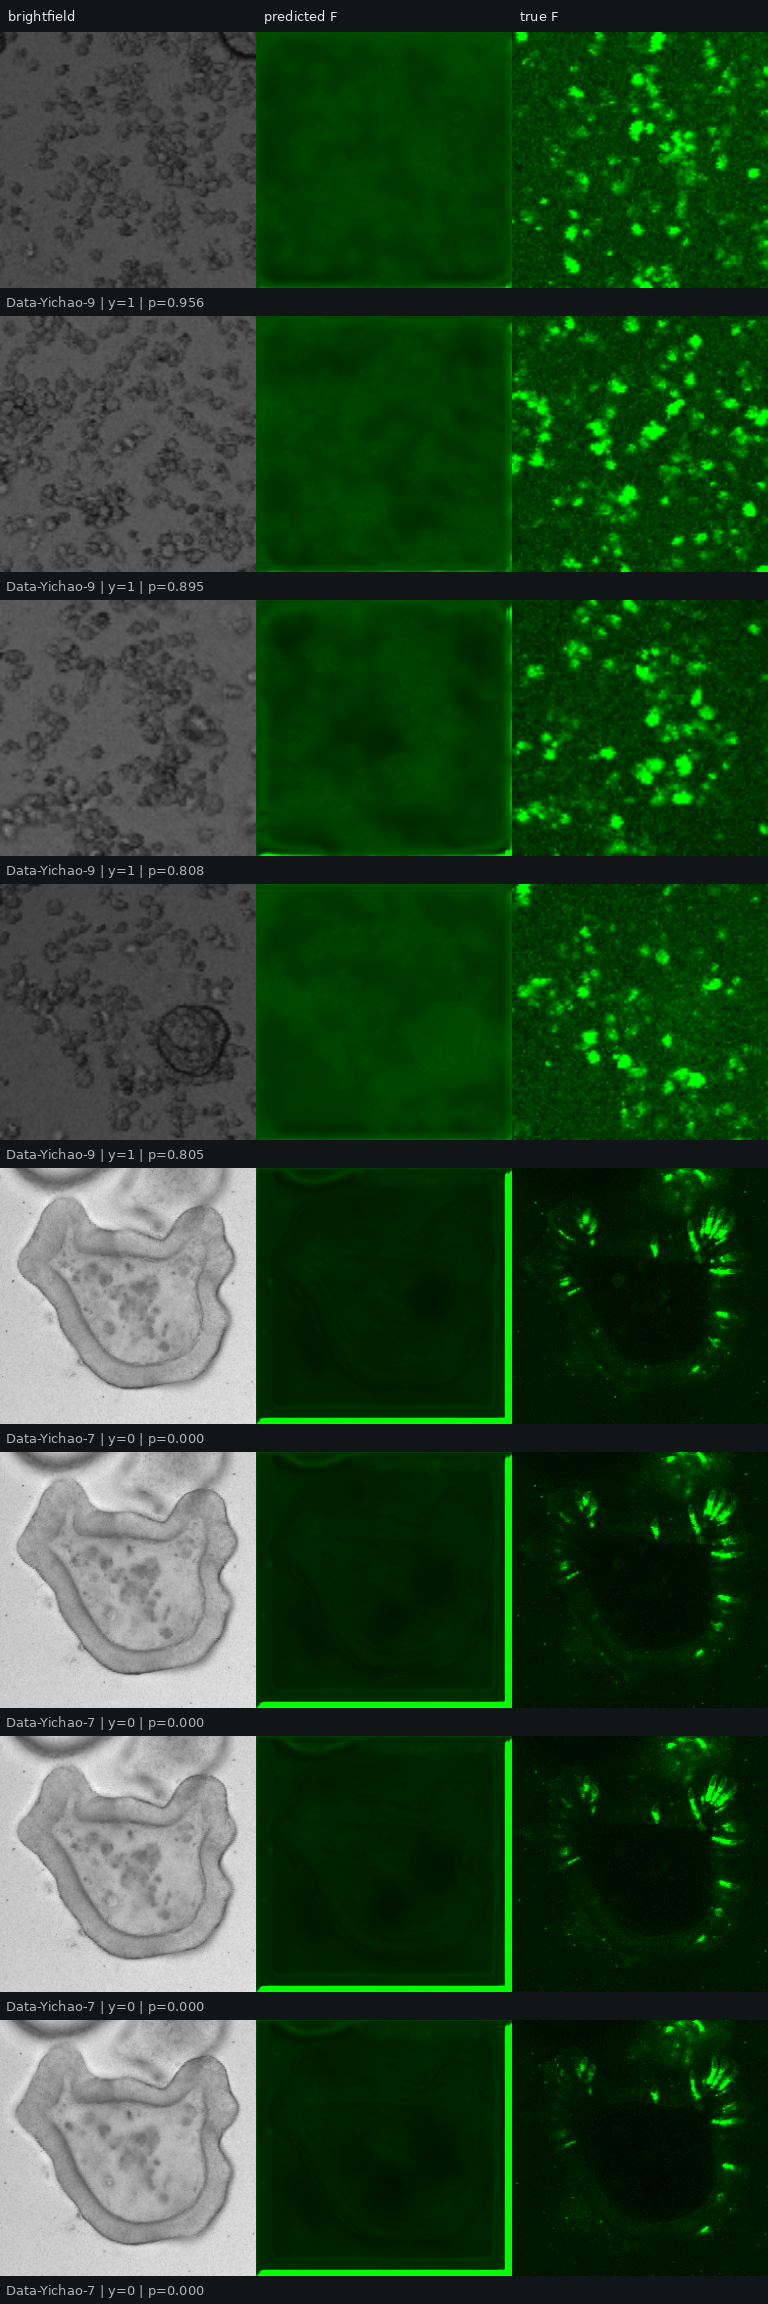
\includegraphics[height=0.82\textheight,keepaspectratio]{figures/fig3_b2f_prediction_examples.png}
\caption{Representative B2F predictions on held-out projected instances. Columns show brightfield input, predicted fluorescence, and true fluorescence.}
\label{fig:b2f-examples}
\end{figure}

The B2F model is a multitask U-Net trained to reconstruct fluorescence images and predict fluorescence scalar endpoints from brightfield. The held-out performance is strong enough to justify using B2F as an auxiliary task in future-expression modeling. The key limitation is class imbalance: only 14 positive instances occur in the B2F test split, making average precision low despite a useful AUROC and intensity correlation.

\section{Feature Explanation}

\begin{figure}[H]
\centering
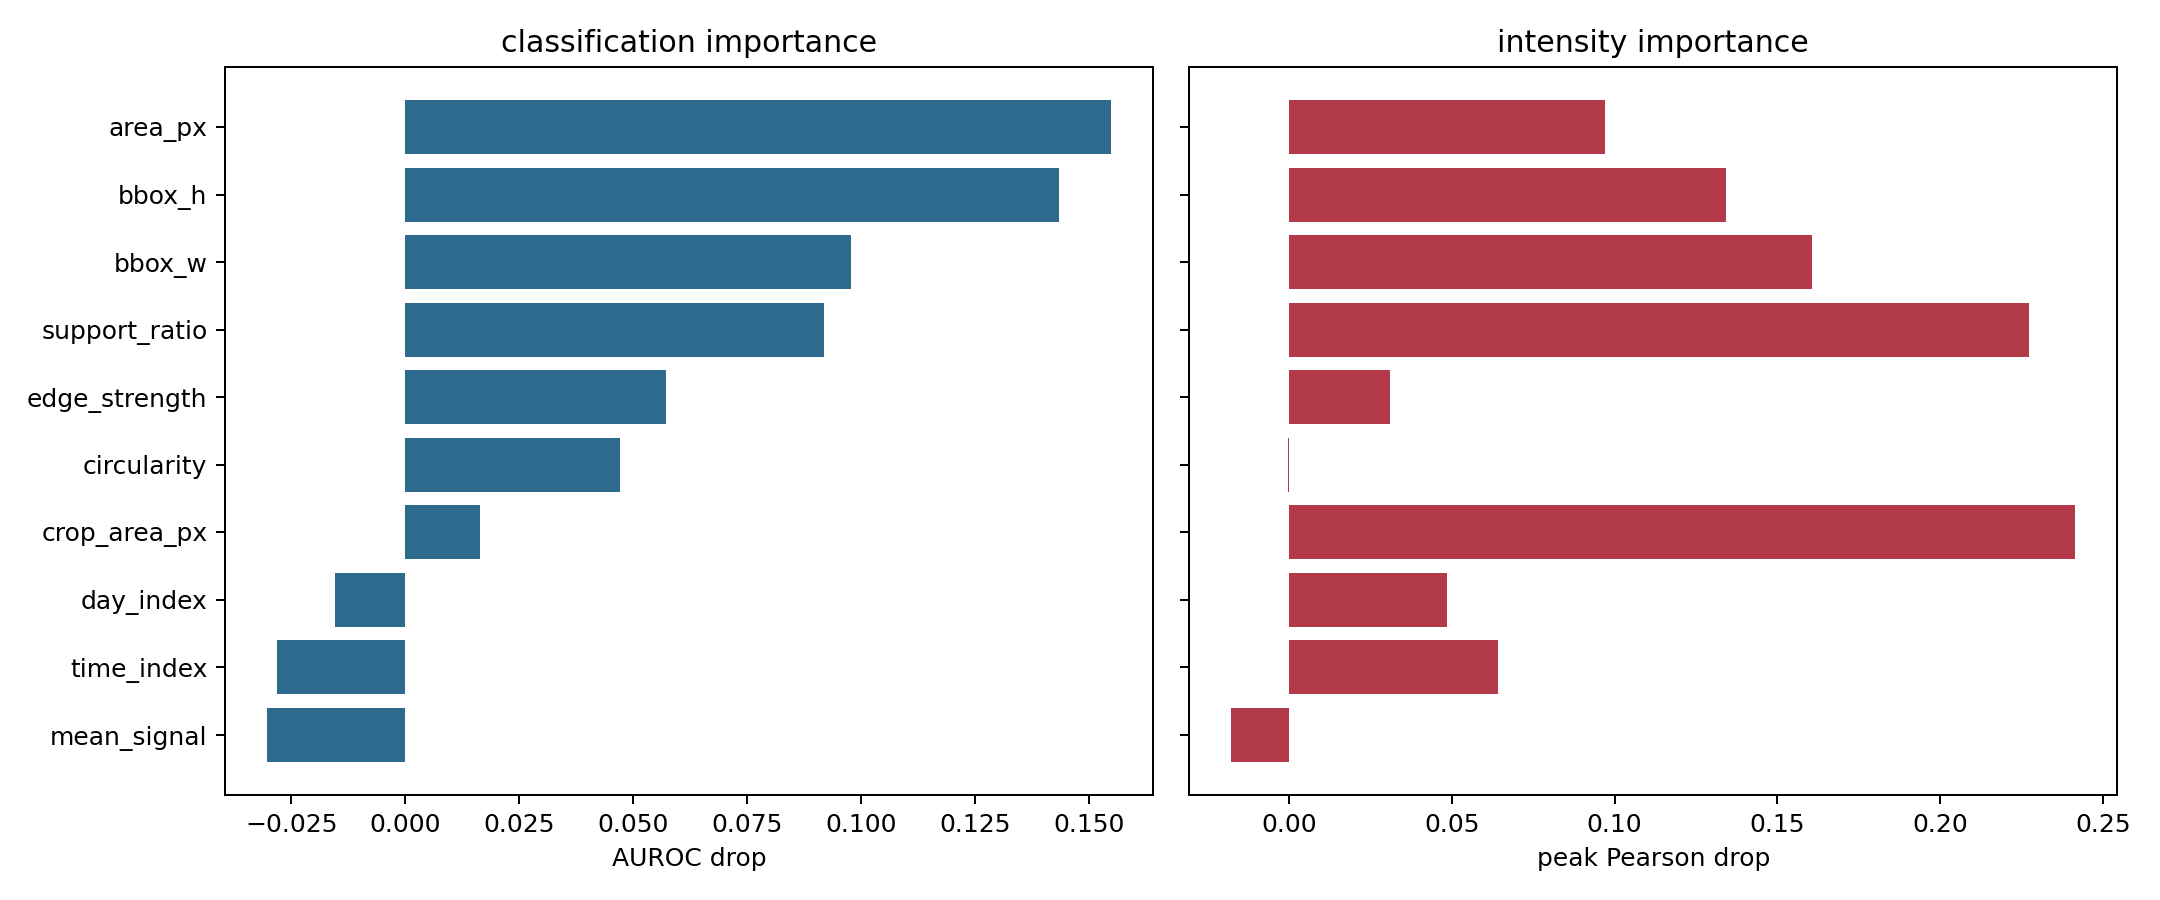
\includegraphics[width=0.92\linewidth]{figures/fig4_feature_importance_summary.png}
\caption{Permutation-based explicit feature importance. Projected area, bounding-box dimensions, support ratio, and edge strength provide the strongest morphology signal.}
\label{fig:feature-importance}
\end{figure}

\begin{figure}[H]
\centering
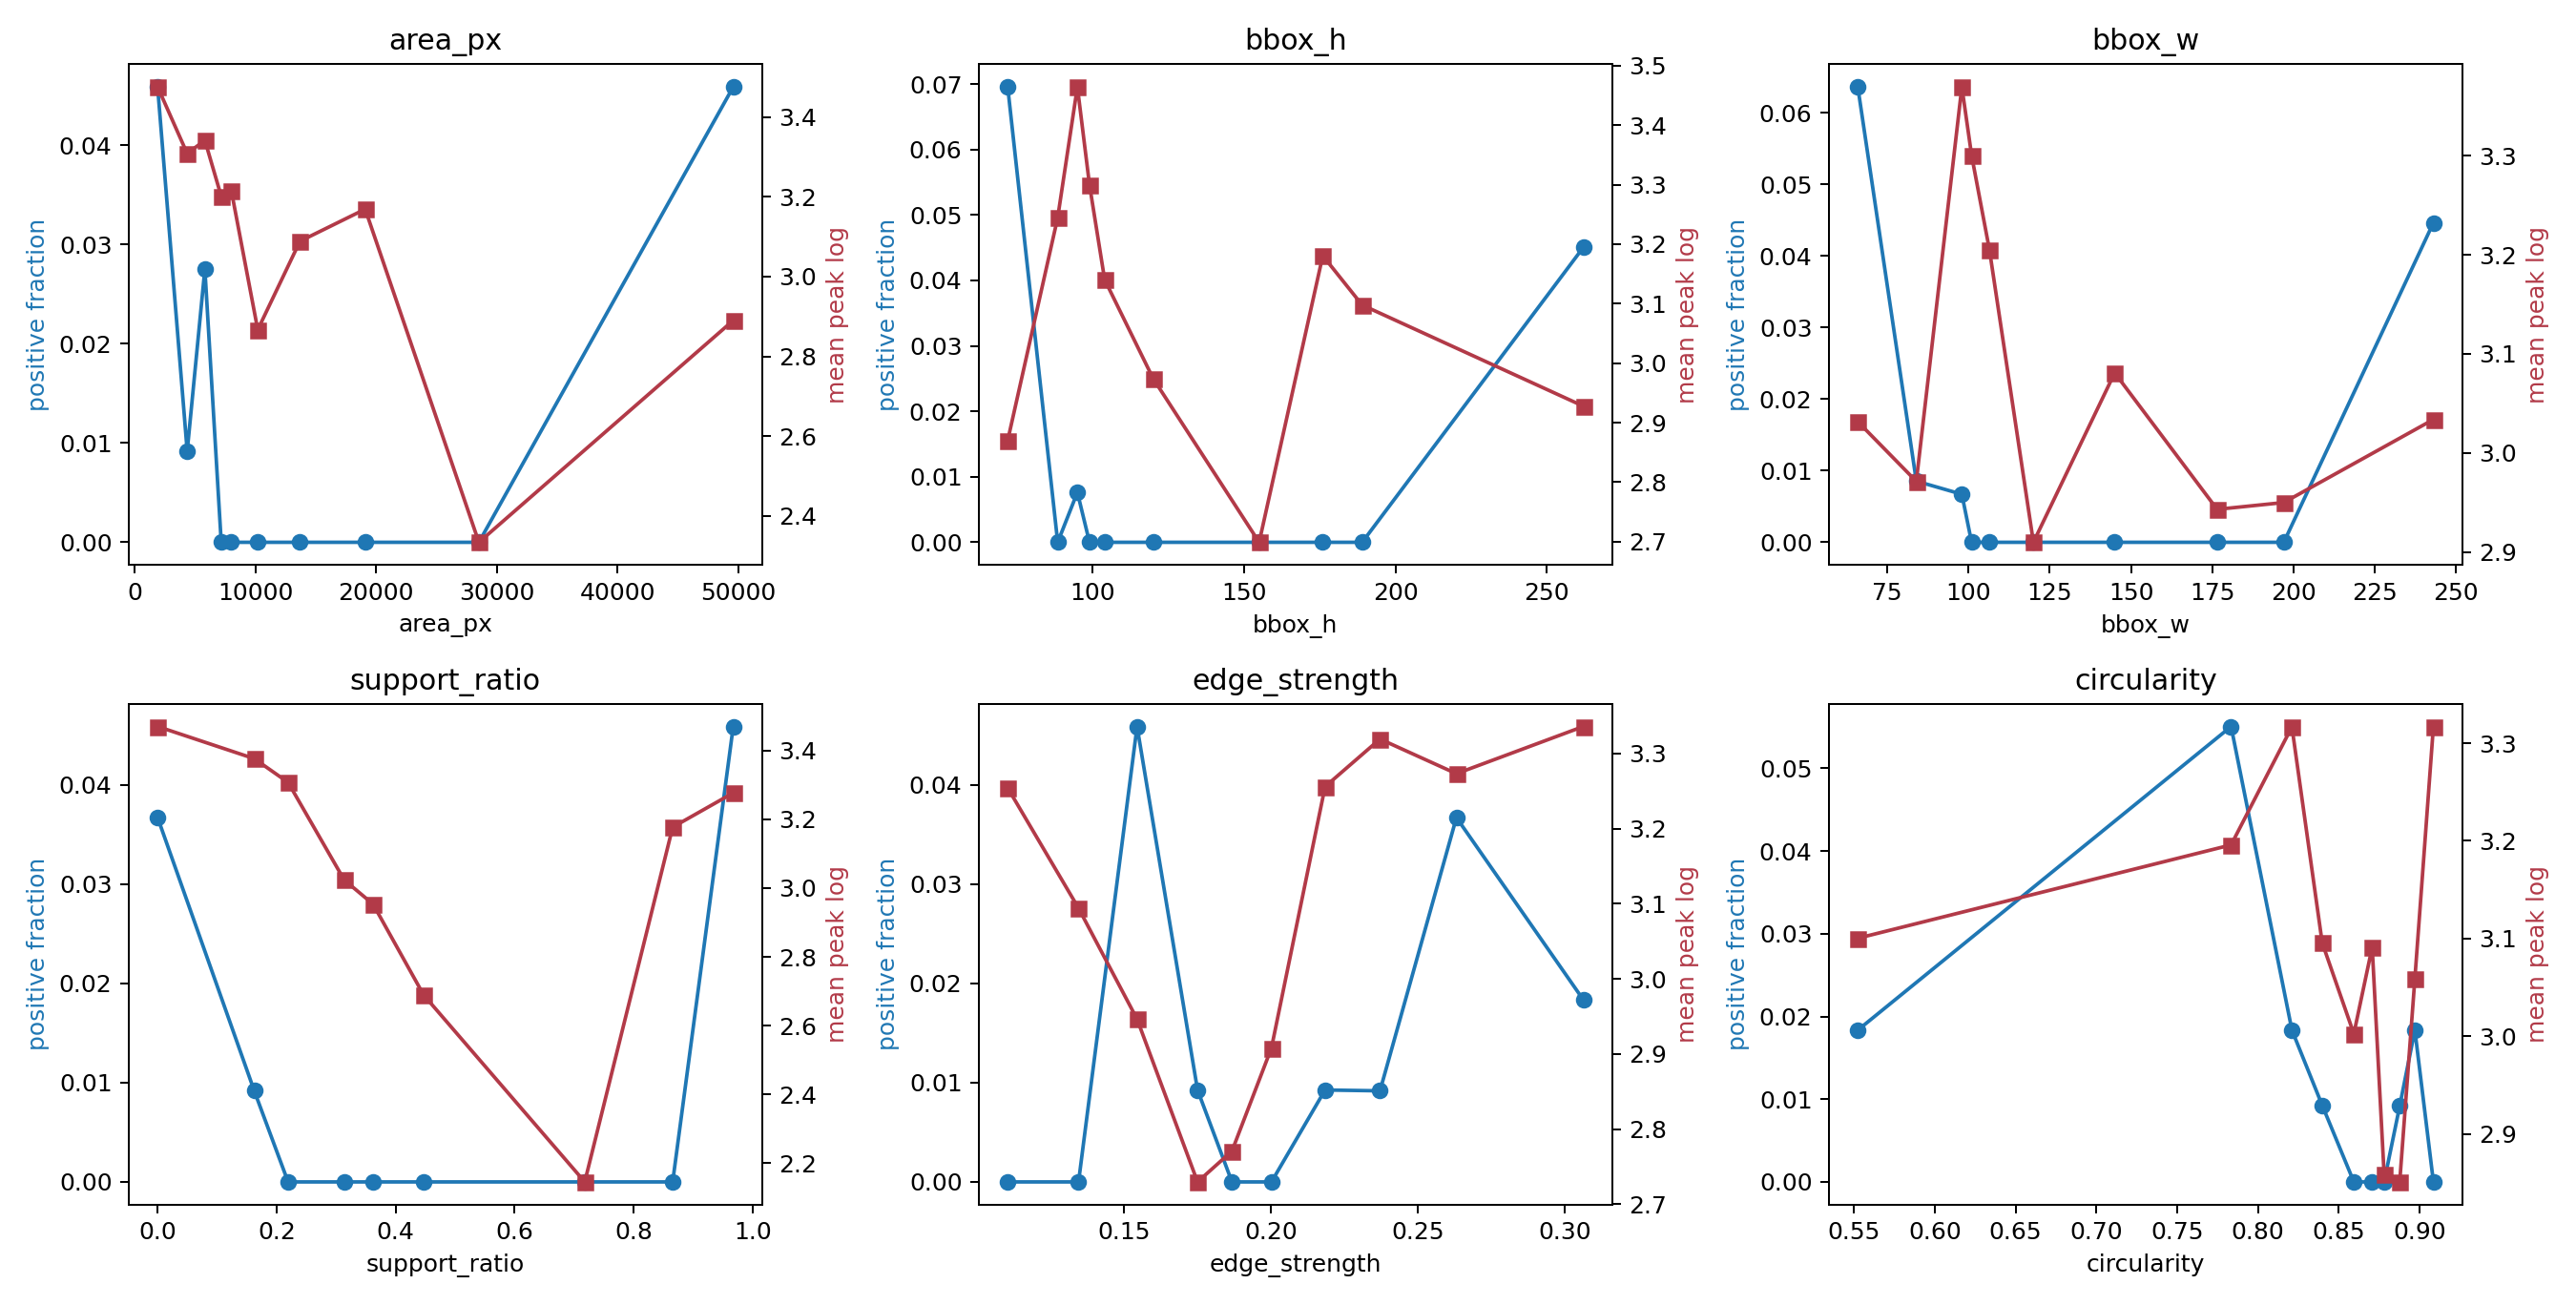
\includegraphics[width=\linewidth]{figures/fig5_feature_trends.png}
\caption{Feature trends across quantiles. Each panel relates explicit morphology features to positive fraction and mean fluorescence peak.}
\label{fig:feature-trends}
\end{figure}

\begin{table}[H]
\centering
\caption{Top explicit morphology features from the B2F feature-analysis model. AUROC drop is measured after feature permutation.}
\begin{tabular}{lcc}
\toprule
Feature & AUROC drop & Peak-correlation drop \\
\midrule
Area & 0.155 & 0.097 \\
Bounding-box height & 0.143 & 0.134 \\
Bounding-box width & 0.098 & 0.161 \\
Support ratio & 0.092 & 0.227 \\
Edge strength & 0.057 & 0.031 \\
Circularity & 0.047 & -0.000 \\
\bottomrule
\end{tabular}
\end{table}

The dominant explanatory features are not arbitrary texture statistics. They are biologically plausible projected morphology cues: size, organoid extent, segmentation support, and boundary strength. These features plausibly encode whether the organoid has reached a state associated with differentiated fluorescent cells, while also helping reject debris and background artifacts that have fluorescence intensity but lack organoid morphology.

\section{Scalar Future-Expression Baseline}

\begin{figure}[H]
\centering
\begin{subfigure}[b]{0.49\linewidth}
\centering
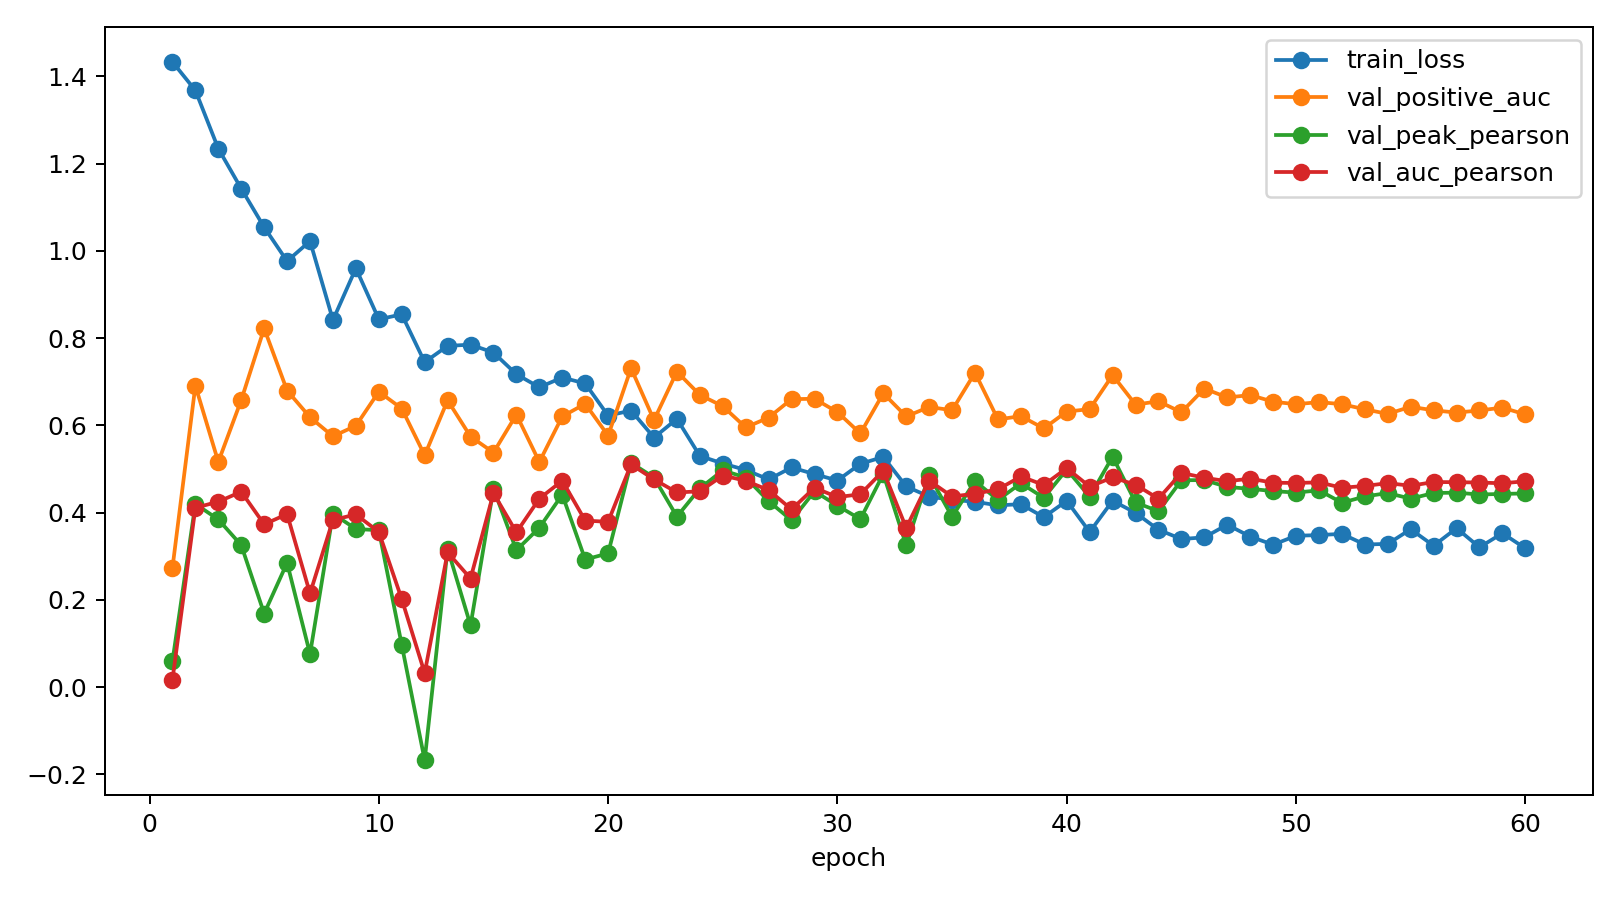
\includegraphics[width=\linewidth]{figures/fig6_scalar_future_training_metrics.png}
\caption{Training curves}
\end{subfigure}
\hfill
\begin{subfigure}[b]{0.49\linewidth}
\centering
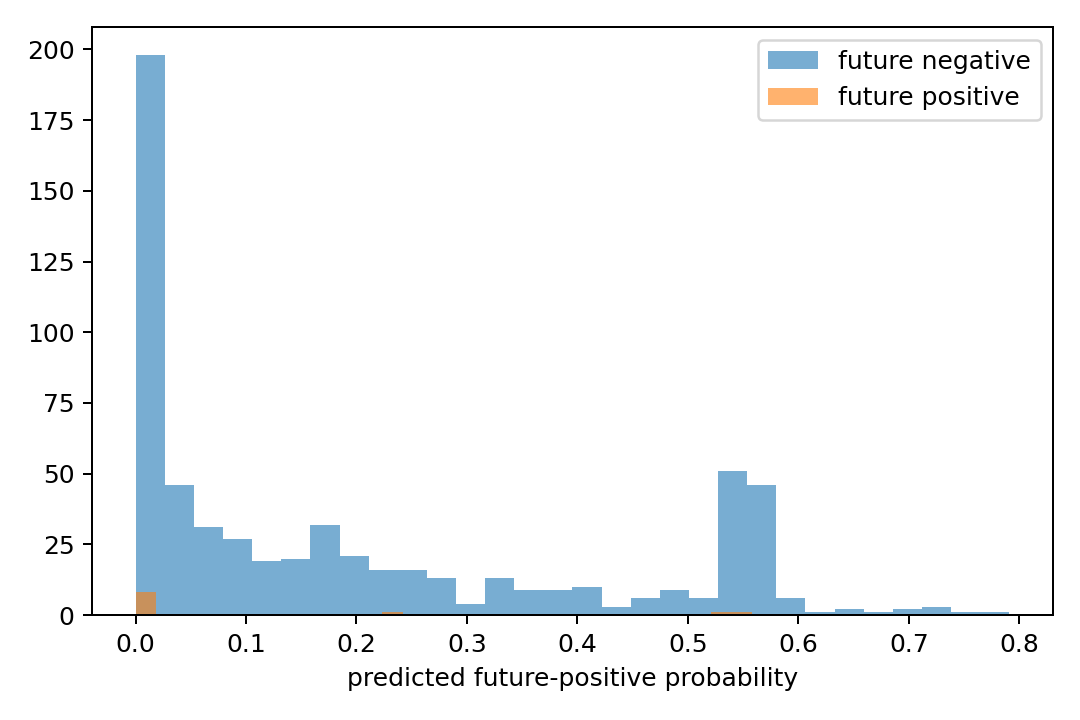
\includegraphics[width=\linewidth]{figures/fig8_scalar_future_score_histogram.png}
\caption{Future-positive scores}
\end{subfigure}

\vspace{0.5em}
\begin{subfigure}[b]{0.72\linewidth}
\centering
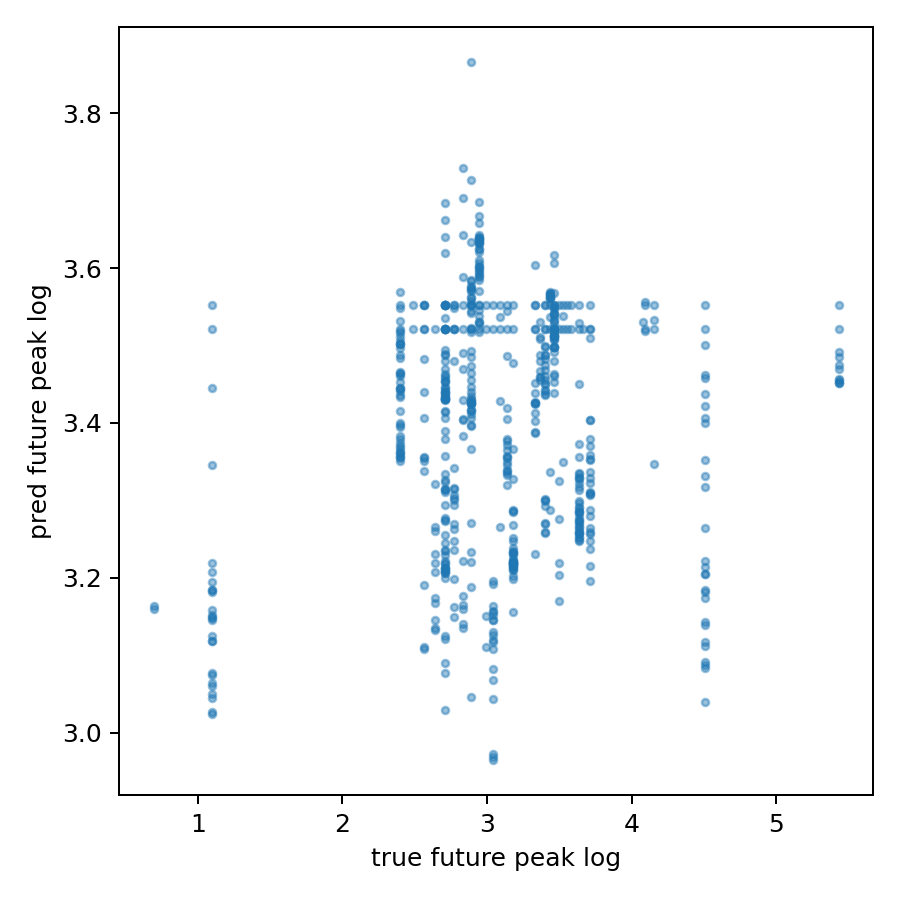
\includegraphics[width=\linewidth]{figures/fig7_scalar_future_peak_scatter.png}
\caption{Future fluorescence peak prediction}
\end{subfigure}
\caption{Scalar-only future-expression baseline visualizations. The held-out test metrics are weak, indicating that this baseline should not be used as the final predictor.}
\label{fig:scalar-future}
\end{figure}

The scalar future baseline predicts future-positive status, future peak fluorescence, and future fluorescence AUC from brightfield prefix embeddings and explicit features. It performs poorly on held-out test data. The most likely causes are rare future-positive examples, approximate track linking, and insufficient supervision from scalar endpoints alone. This failure mode is useful: it motivates training a joint model that predicts dense future fluorescence images, not only scalar labels.

\section{Joint B2F/Future Model}

\begin{figure}[H]
\centering
\begin{subfigure}[b]{0.49\linewidth}
\centering
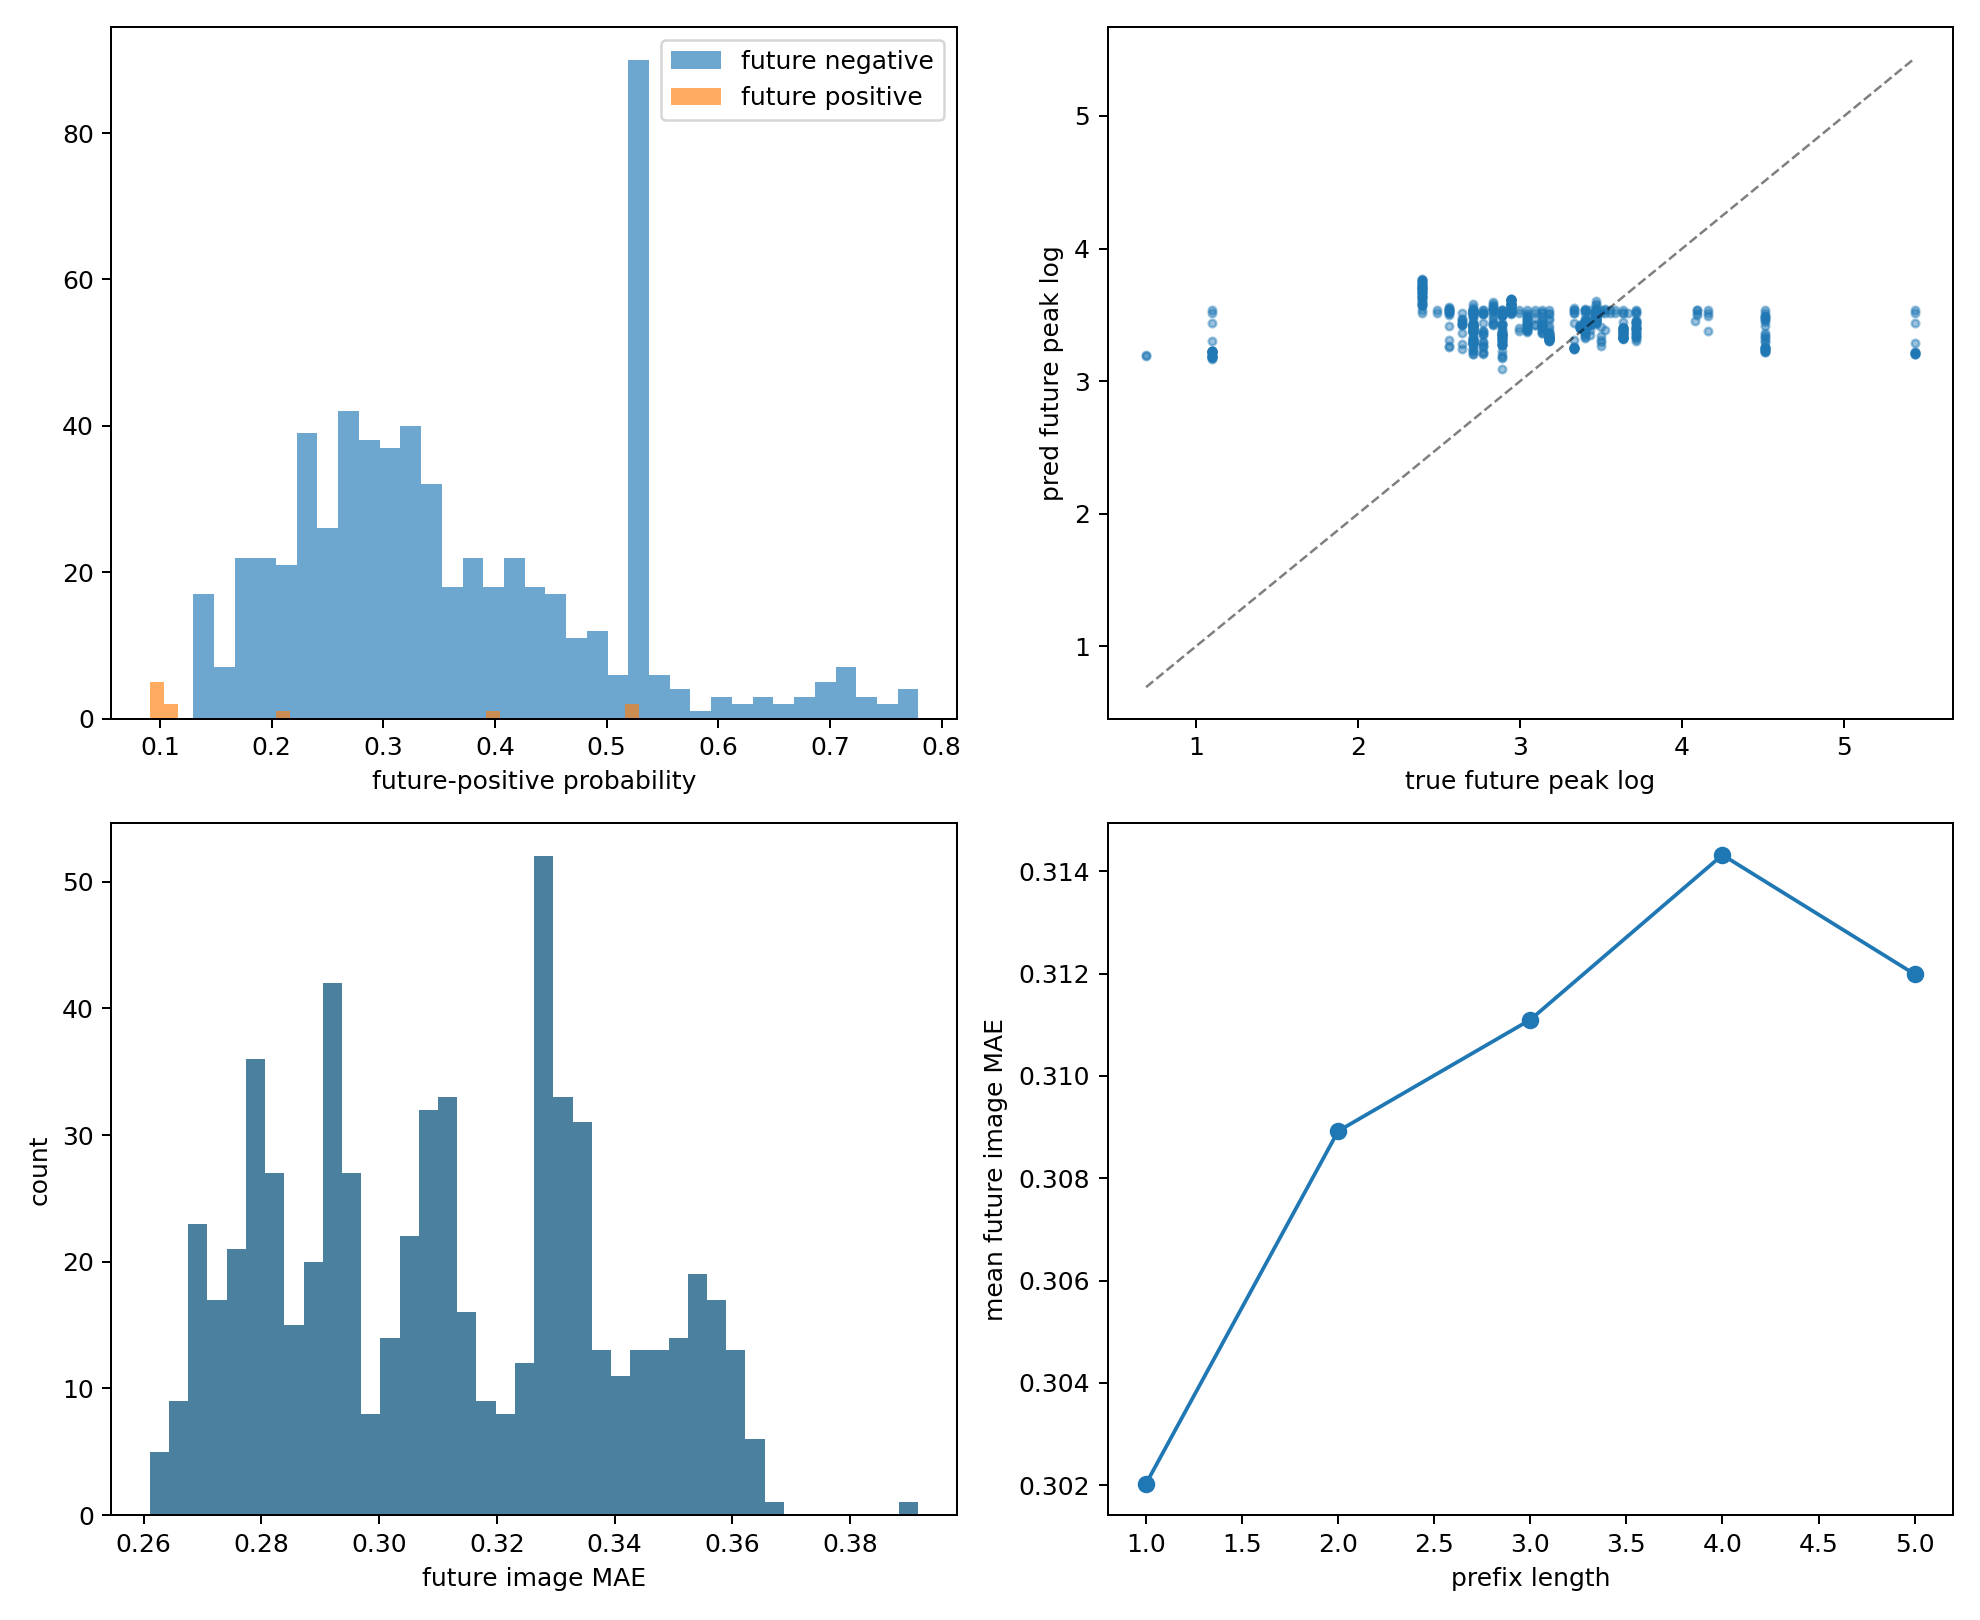
\includegraphics[width=\linewidth]{figures/fig10_joint_future_summary.png}
\caption{Final joint test summary}
\end{subfigure}
\hfill
\begin{subfigure}[b]{0.49\linewidth}
\centering
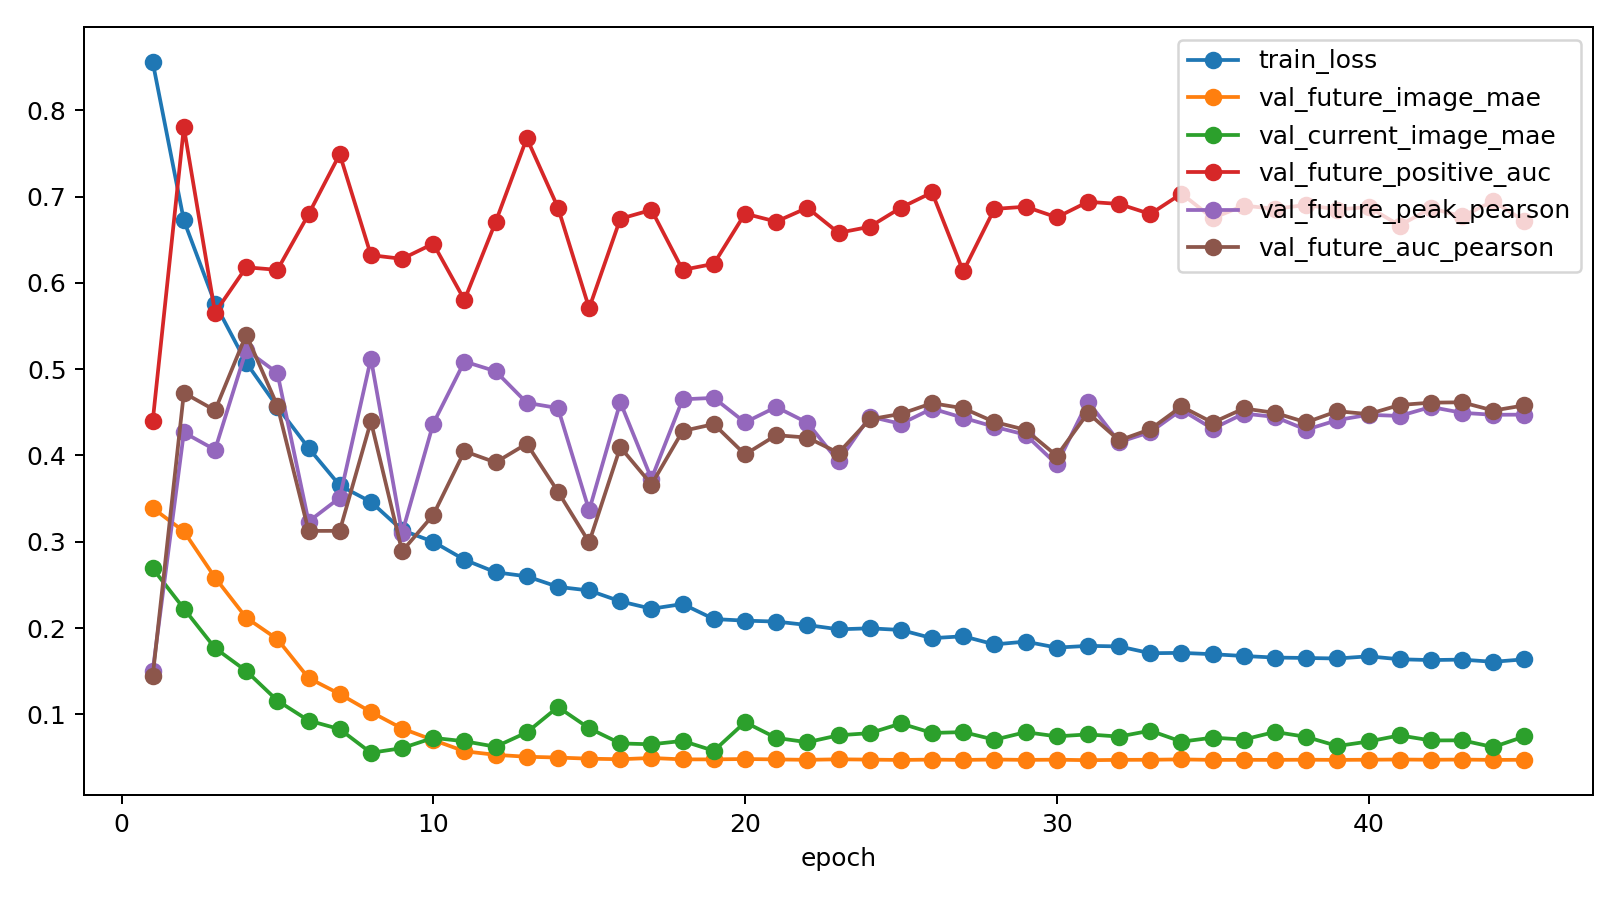
\includegraphics[width=\linewidth]{figures/fig11_joint_training_metrics.png}
\caption{Joint training curves}
\end{subfigure}
\caption{Joint model quantitative visualizations. Validation losses improved during training, but the selected best validation-AUROC checkpoint did not generalize to the held-out future test split.}
\label{fig:joint-summary}
\end{figure}

\begin{figure}[H]
\centering
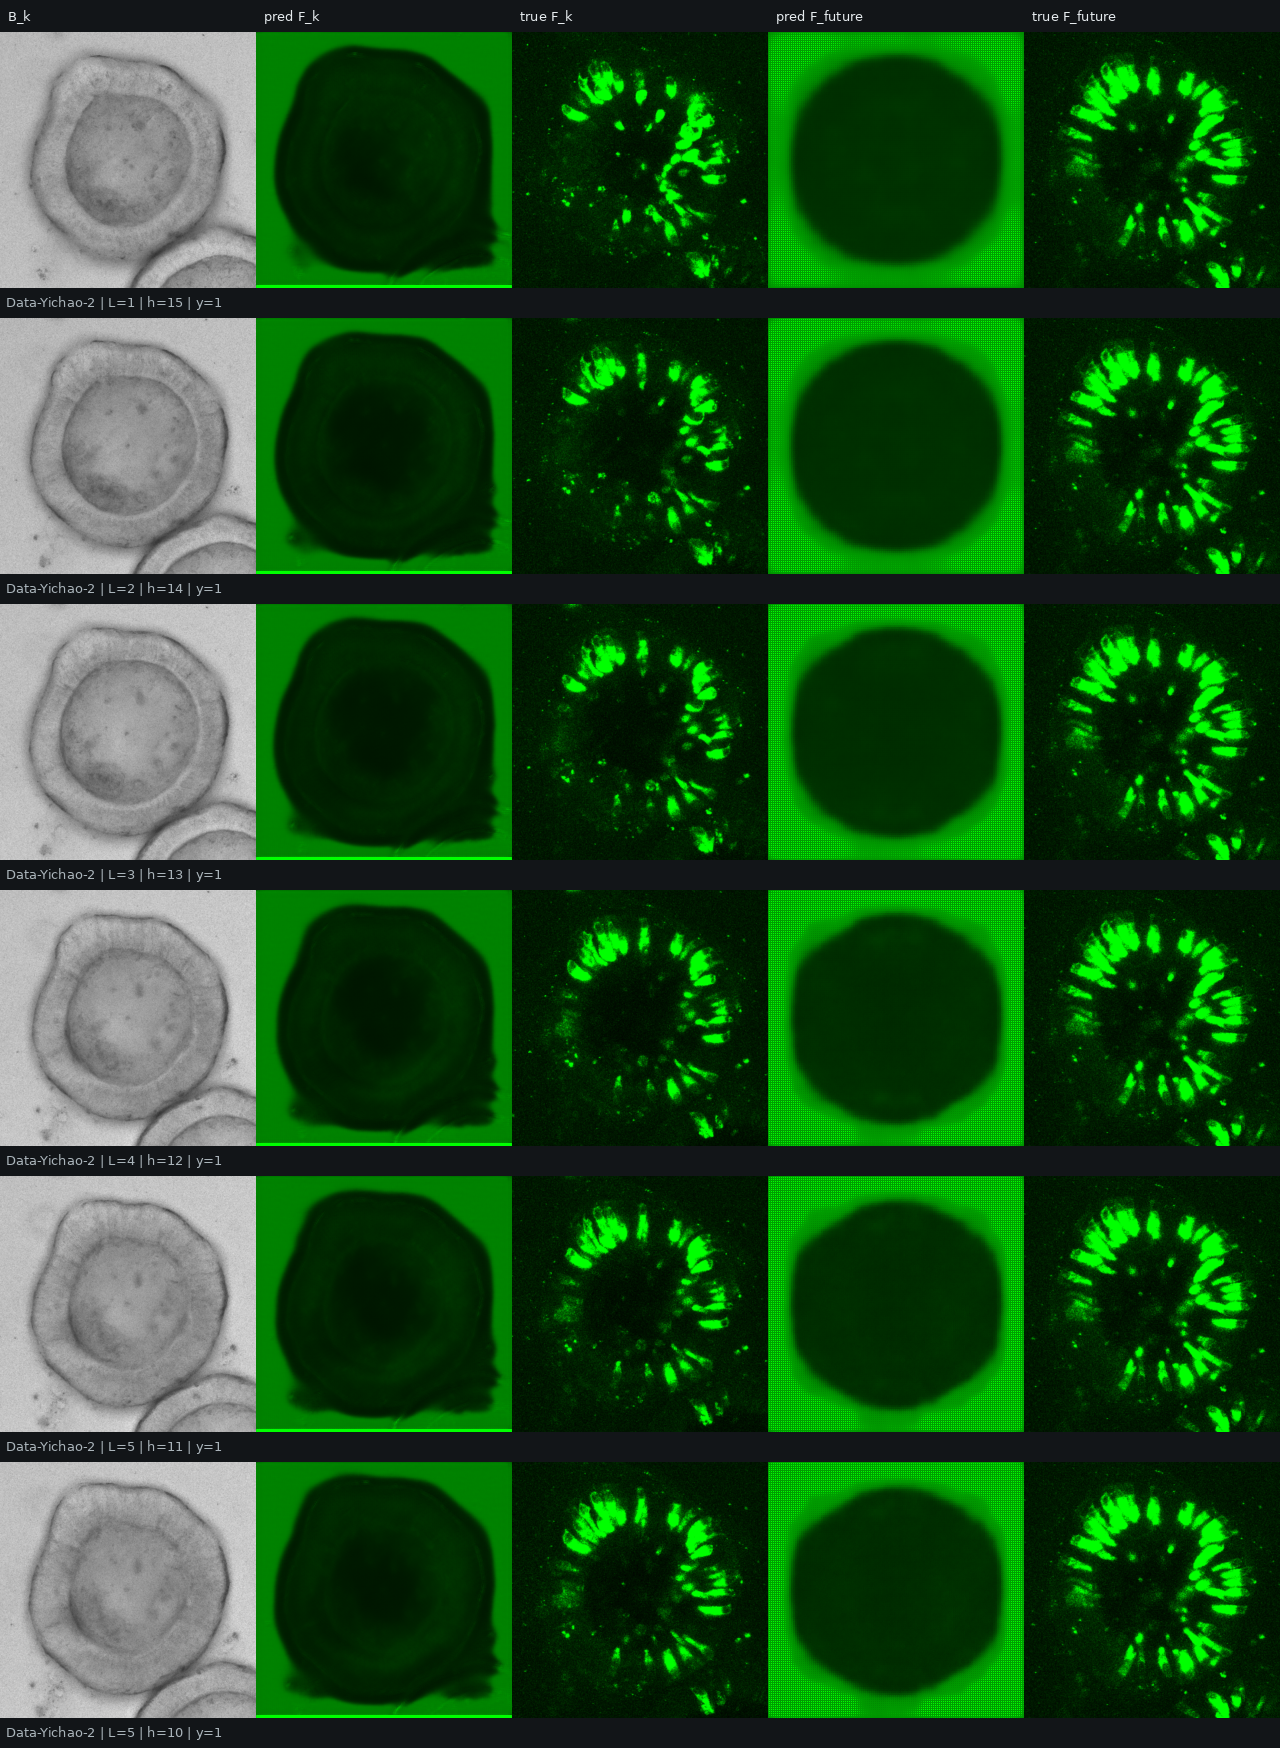
\includegraphics[height=0.82\textheight,keepaspectratio]{figures/fig9_joint_test_predictions.png}
\caption{Final held-out test prediction panel from the joint model. Columns show current brightfield input, auxiliary predicted current fluorescence, true current fluorescence, predicted future fluorescence, and true future fluorescence.}
\label{fig:joint-test-panel}
\end{figure}

\begin{figure}[H]
\centering
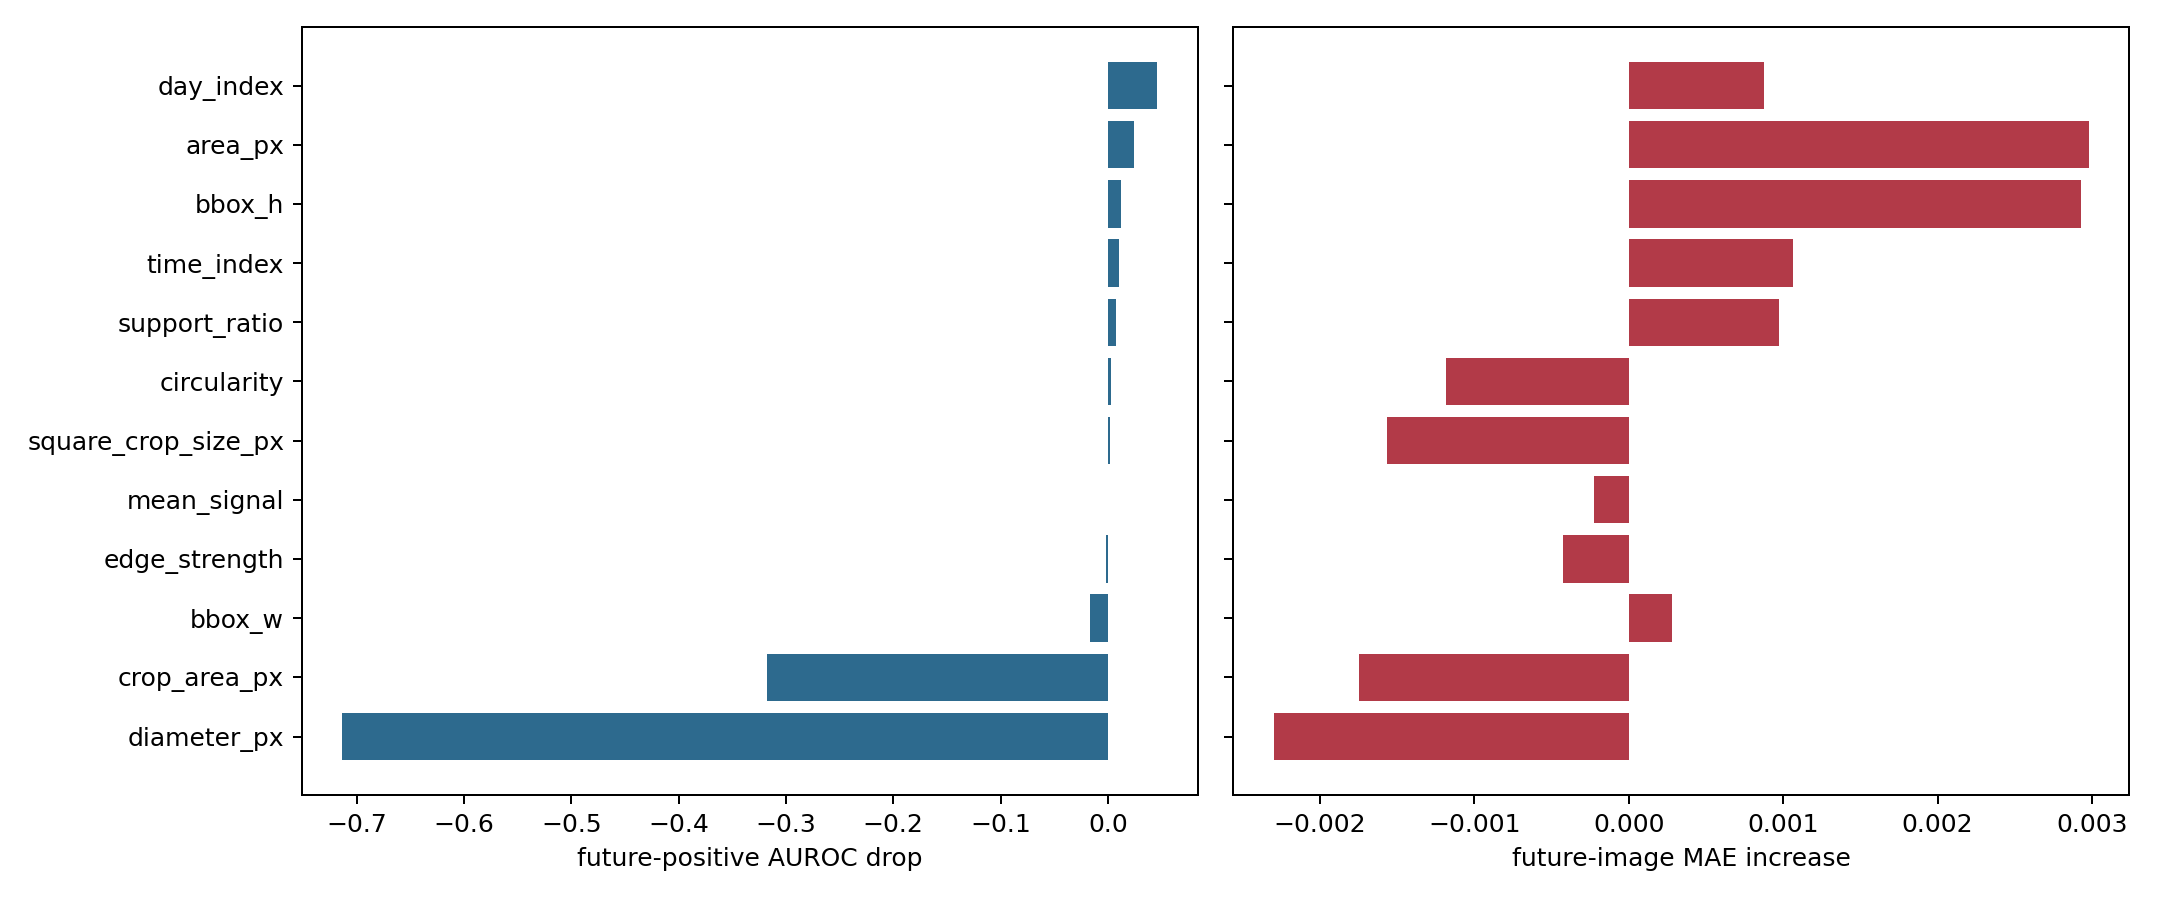
\includegraphics[width=0.92\linewidth]{figures/fig12_joint_feature_ablation.png}
\caption{Joint model feature-ablation summary on the held-out future test split. Day/time and size features show the largest positive AUROC drops, but overall held-out future performance remains weak.}
\label{fig:joint-feature-ablation}
\end{figure}

The joint model is trained in the separate output directory \path{\outputroot/stage3_joint_b2f_future}. It achieved strong-looking validation performance during training, including validation future-image MAE near 0.047 and validation future-positive AUROC frequently above 0.65. However, the final held-out test metrics remain weak: future-image MAE is 0.3112, future-positive AUROC is 0.223, future-positive AP is 0.0127, future-peak Pearson correlation is -0.049, and future-AUC Pearson correlation is 0.075. The best validation-AUROC checkpoint was epoch 2, which suggests unstable model selection under strong dataset/track split effects and rare positives. This is an important negative result: dense future-image supervision alone does not solve early future-expression prediction with the current track construction and split.

\section{Interpretation and Next Steps}

The completed experiments support three conclusions:

\begin{enumerate}
\item Same-time B2F is feasible on projected complete/non-edge organoid crops.
\item Explicit morphology explains a meaningful part of fluorescence distinction, especially projected size, bounding-box dimensions, segmentation support, and boundary strength.
\item Scalar-only early future prediction and the first dense joint future model are both weak on the held-out future test split.
\end{enumerate}

The next decision point is not model complexity; it is data and target reliability. The current results suggest that early future prediction needs better track verification, horizon-specific evaluation, and possibly a target policy based on the peak future fluorescence frame rather than the last available future frame. Same-time B2F remains the strongest validated component and should be retained as an auxiliary or pretraining task.

\section{Methods Summary}

The projected dataset was built from complete non-edge organoid instances. Brightfield and fluorescence crops were resized to $256 \times 256$. Same-time B2F was trained with paired brightfield and fluorescence crops. Future samples were constructed from linked time-series tracks using a prefix $B_{0:k}$ and a future target $F_{p>k}$. The first future model used a CNN/GRU feature encoder with scalar heads. The joint model adds dense future fluorescence image prediction and an auxiliary same-time B2F branch.

\section{Reproducibility}

The primary source code lives under:

\begin{center}
\small
\path{/home/lachlan/ProjectsLFS/OrganoidAgent/differentiation_prediction/yichao_future_expression}
\end{center}

The research prompt and mathematical plan are saved at:

\begin{center}
\small
\path{/home/lachlan/ProjectsLFS/OrganoidAgent/references/Yichao/joint_b2f_future_expression_research_prompt.md}
\end{center}

The consolidated previous-run report is saved at:

\begin{center}
\small
\path{/home/lachlan/ProjectsLFS/OrganoidAgent/analysis-outputs/yichao_future_expression/previous_run_evaluation/previous_run_report.md}
\end{center}

\begin{thebibliography}{9}

\bibitem{isola2017pix2pix}
Isola, P., Zhu, J.-Y., Zhou, T. and Efros, A. A.
Image-to-image translation with conditional adversarial networks.
\textit{CVPR} (2017).
\url{https://arxiv.org/abs/1611.07004}

\bibitem{fnet}
Allen Cell Modeling.
Pytorch-FNet: label-free prediction of fluorescence images from transmitted-light microscopy.
\url{https://allencellmodeling.github.io/pytorch_fnet/}

\bibitem{shi2015convlstm}
Shi, X. et al.
Convolutional LSTM network: A machine learning approach for precipitation nowcasting.
\url{https://arxiv.org/abs/1506.04214}

\bibitem{vafaeikia2020mtl}
Vafaeikia, P., Namdar, K. and Khalvati, F.
A brief review of deep multi-task learning and auxiliary task learning.
\url{https://arxiv.org/abs/2007.01126}

\end{thebibliography}

\end{document}
